\documentclass[tikz, border=10mm]{standalone}
\usepackage{tikz}
\usetikzlibrary{positioning, calc, arrows.meta, chains, fit, shapes, backgrounds}
% nn_blocks.tex
% Defines styles for neural network blocks using TikZ
% Now supports Hybrid 2D/3D Visualization with PlotNeuralNet

% --- PlotNeuralNet Integration ---
% We assume Ball.sty, Box.sty, RightBandedBox.sty are in the same directory
\usepackage{Ball}
\usepackage{Box}
\usepackage{RightBandedBox}

% PlotNeuralNet Init Definitions (from init.tex)
\usetikzlibrary{quotes,arrows.meta}
\usetikzlibrary{positioning}
\def\edgecolor{rgb:blue,4;red,1;green,4;black,3}
\newcommand{\midarrow}{\tikz \draw[-Stealth,line width =0.8mm,draw=\edgecolor] (-0.3,0) -- ++(0.3,0);}

% Define PlotNeuralNet Colors (Standard Palette)
\definecolor{ConvColor}{rgb}{0.98,0.81,0.69}  % Apricot/Orange
\definecolor{ConvReluColor}{rgb}{0.98,0.81,0.69}
\definecolor{PoolColor}{rgb}{0.8,0.33,0.33}   % Redish
\definecolor{UnpoolColor}{rgb}{0.6,0.7,0.9}   % Blueish
\definecolor{FcColor}{rgb}{0.6,0.2,0.8}       % Purple
\definecolor{FcReluColor}{rgb}{0.6,0.2,0.8}
\definecolor{SoftmaxColor}{rgb}{0.9,0.9,0.6}  % Yellowish
\definecolor{SumColor}{rgb}{0.9,0.9,0.9}      % Gray

% Custom colors for our specific blocks
\definecolor{ResBlockColor}{rgb}{0.85,0.92,1.0} % Light Blue
\definecolor{EmbedColor}{rgb}{0.95,0.95,0.8}    % Light Yellow
\definecolor{TransColor}{rgb}{0.8,0.9,0.8}      % Light Green

% --- NNTikZ 2D Styles (Matched to EDSR Style) ---
\usetikzlibrary{positioning, chains, shapes.geometric, fit, shapes, arrows.meta, calc, backgrounds, shadows}

\tikzset{
    >=LaTeX, 
    very thick,
    node distance=1.0cm and 1.2cm,
    % Basic Arrow
    arrow/.style={
        ->,
        very thick,
        draw=black!80,
        rounded corners=0.2cm
    },
    % Dashed Skip Connection
    skip/.style={
        arrow,
        dashed,
        draw=blue!60
    },
    % Grouping Block (Background Box)
    block/.style={
        rectangle,
        fill=gray!10,
        rounded corners=3mm,
        draw=black!60,
        very thick,
        inner sep=0.8em,
        drop shadow={opacity=0.15}
    },
    nntikz_block/.style={block}, % Alias
    % General Layer
    layer/.style={
        rectangle,
        fill=white!10,
        rounded corners=1mm,
        inner xsep=0.6em,
        inner ysep=0.6em,
        minimum height=3.0em,
        align=center,
        draw=black!80,
        very thick,
        drop shadow={opacity=0.2, shadow xshift=1mm, shadow yshift=-1mm}
    },
    nntikz_layer/.style={layer}, % Alias
    % Specific Layer Types
    conv/.style={
        layer,
        fill=orange!10,
        draw=orange!80!black
    },
    relu/.style={
        layer,
        fill=yellow!10,
        draw=yellow!80!black,
        minimum height=2.5em
    },
    pool/.style={
        layer,
        fill=red!10,
        draw=red!80!black
    },
    up/.style={
        layer,
        fill=purple!10,
        draw=purple!80!black
    },
    res/.style={ % Residual Block or similar
        layer,
        fill=blue!5,
        draw=blue!80!black
    },
    op/.style={ % Other operations
        layer,
        fill=green!10,
        draw=green!80!black
    },
    % Input/Output
    input/.style={ 
        circle,
        minimum width=3.0em,
        draw=black!80,
        fill=gray!20,
        thick,
        align=center,
        drop shadow={opacity=0.2}
    },
    io/.style={input}, % Alias
    % Summation
    sum/.style={
        circle,
        draw=black!80,
        fill=white,
        inner sep=0pt,
        minimum size=1.2em,
        node contents={+}
    }
}


\begin{document}
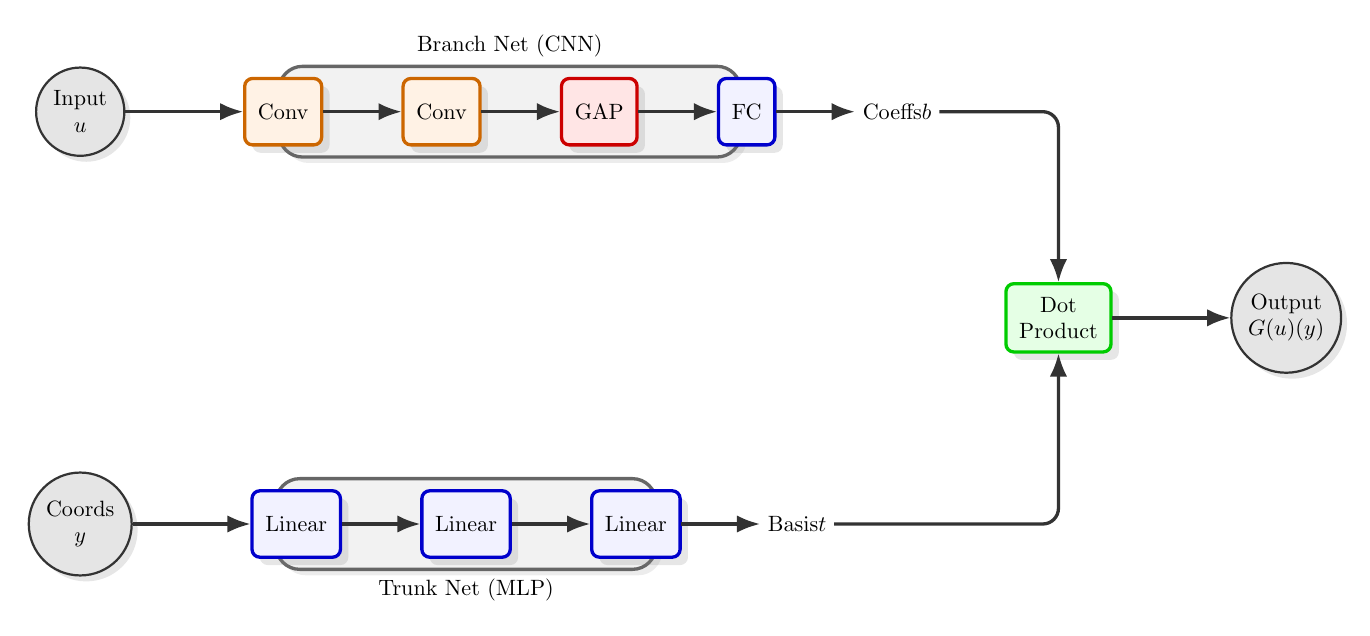
\begin{tikzpicture}[
    node distance=1.5cm,
    every node/.style={scale=0.8, transform shape}
]

% --- Branch Net (Top) ---
% Input
\node[io] (in_u) {Input\\$u$};

% Layers (Flat layout)
\node[conv, right=of in_u] (c1) {Conv};
\node[conv, right=1.0cm of c1] (c2) {Conv};
\node[pool, right=1.0cm of c2] (gap) {GAP};
\node[res, right=1.0cm of gap] (fc) {FC};

% Output of Branch
\node[right=1.0cm of fc] (b_out) {Coeffs\\$b$};

% Connections
\draw[arrow] (in_u) -- (c1);
\draw[arrow] (c1) -- (c2);
\draw[arrow] (c2) -- (gap);
\draw[arrow] (gap) -- (fc);
\draw[arrow] (fc) -- (b_out);

% Grouping Box
\begin{scope}[on background layer]
    \node[block, fit=(c1) (fc), label=above:Branch Net (CNN)] (branch_box) {};
\end{scope}

% --- Trunk Net (Bottom) ---
% Input (Aligned below u)
\node[io, below=4.0cm of in_u] (in_y) {Coords\\$y$};

% Layers
\node[res, right=of in_y] (l1) {Linear};
\node[res, right=1.0cm of l1] (l2) {Linear};
\node[res, right=1.0cm of l2] (l3) {Linear};

% Output of Trunk
\node[right=1.0cm of l3] (t_out_node) {Basis\\$t$};

% Connections
\draw[arrow] (in_y) -- (l1);
\draw[arrow] (l1) -- (l2);
\draw[arrow] (l2) -- (l3);
\draw[arrow] (l3) -- (t_out_node);

% Grouping Box
\begin{scope}[on background layer]
    \node[block, fit=(l1) (l3), label=below:Trunk Net (MLP)] (trunk_box) {};
\end{scope}

% --- Fusion ---
\coordinate (mid) at ($(b_out)!0.5!(t_out_node)$);
\node[op, right=2.0cm of mid] (dot) {Dot\\Product};

% Output
\node[io, right=of dot] (out) {Output\\$G(u)(y)$};

% Fusion Connections
\draw[arrow] (b_out) -| (dot);
\draw[arrow] (t_out_node) -| (dot);
\draw[arrow] (dot) -- (out);

\end{tikzpicture}
\end{document}